\documentclass[11pt]{article}

% --------------------------------------------------
% Packages
% --------------------------------------------------
\usepackage[margin=1in]{geometry}
\usepackage{amsmath, amssymb, amsthm}
\usepackage{mathtools}
\usepackage{graphicx}
\usepackage{float}
\usepackage{enumitem}
\usepackage{hyperref}
\usepackage{xcolor}
\usepackage{tikz}
\usetikzlibrary{arrows.meta, positioning, calc}

% Pseudocode and algorithms
\usepackage{algorithm}
\usepackage{algpseudocode}

% Better fonts (optional)
\usepackage{lmodern}

% --------------------------------------------------
% Hyperref setup
% --------------------------------------------------
\hypersetup{
	colorlinks=true,
	linkcolor=blue,
	citecolor=blue,
	urlcolor=blue
}

% --------------------------------------------------
% Theorem-like environments
% --------------------------------------------------
\theoremstyle{definition}
\newtheorem{definition}{Definition}[section]
\newtheorem{theorem}{Theorem}[section]
\newtheorem{claim}{Claim}[section]
\newtheorem{remark}{Remark}[section]

\theoremstyle{proof}
% Proof environment is built-in via amsthm

% --------------------------------------------------
% Custom commands
% --------------------------------------------------
\newcommand{\Gen}{\mathsf{Gen}}
\newcommand{\Enc}{\mathsf{Enc}}
\newcommand{\Dec}{\mathsf{Dec}}
\newcommand{\Sig}{\mathsf{Sig}}
\newcommand{\Ver}{\mathsf{Ver}}
\newcommand{\negl}{\mathsf{negl}}

% --------------------------------------------------
% Document
% --------------------------------------------------
\begin{document}
	
	\title{Public Key Crypto notes - 05}
	\author{By contributors}
	\date{March 09. 2026}
	\maketitle
	
	% --------------------------------------------------
	\section{Various theorems}
	% --------------------------------------------------
	
	\begin{theorem}
		Computing $x$ from $N, e$ and $x^e \pmod{N}$ is as hard as computing $lsb(x)$.
	\end{theorem}
	
	\begin{proof}
		Let $A$ be an adversary such that $A(r^e \pmod{N}) = lsb(r)$ for any $r \in \mathbb{Z}_N^*$. We use $A$ to recover $x$ from $x^e \pmod{N}$:
		\begin{enumerate}
			\item $lsb(x)$ is given by $A(x^e \pmod{N})$.
			\item To compute $2nd(x)$ (which is the second least significant bit), let $y = x^e \pmod{N}$.
			\item Cases:
			\begin{enumerate}
				\item $lsb(0) \rightarrow x$ is even $\rightarrow 2nd(x) = lsb(\frac{x}{2})$. Note that $A(\frac{y}{2^e}) = A((\frac{x}{2})^e) = 2nd(x)$.
				\item $lsb(x) = 1 \rightarrow x$ is odd. $\frac{x}{2} \pmod{N} = \frac{x+N}{2}$ (since we are working in modular arithmetic). We are trying to find:
				\begin{align}
					lsb(\frac{x}{2}) \pmod{N} &= 2nd(x+N) = \\
					&= 2nd(x) + 2nd(N) + 1 \pmod{2}
				\end{align}
				So:
				\begin{align}
					2nd(x) &= lsb(\frac{x}{2} \pmod{N}) + 2nd(N) + 1 \pmod{2} = \\
					&= A(\frac{y}{2^e} \pmod{N}) + 2nd(N) + 1 \pmod{2}
				\end{align}
			\end{enumerate}
		\end{enumerate}
	\end{proof}
	
	\begin{remark}
		If $m \in \{0, 1\}$ and $c = (r || m)^e \pmod{N}$ where $r$ is a random integer of bit size $2n-1$, then it is a CPA-secure encryption.
	\end{remark}
	
	\section{Padding schemes}
	
	\subsection{RSA PKCS\#1 v1.5: Padded RSA}
	
	$\hat{m} = (0,\_,0 || r || 0,\_,0 || m)$ with random $r$ ($\hat{m}$ is the padded message).
	
	This scheme has some security disadvantages\footnote{\url{https://medium.com/@c0D3M/bleichenbacher-attack-explained-bc630f88ff25}}.
	
	\subsection{RSA-OAEP-optimal asymmetric encryption padding}
	
	Let $G, H$ be two secure hash functions.
	
	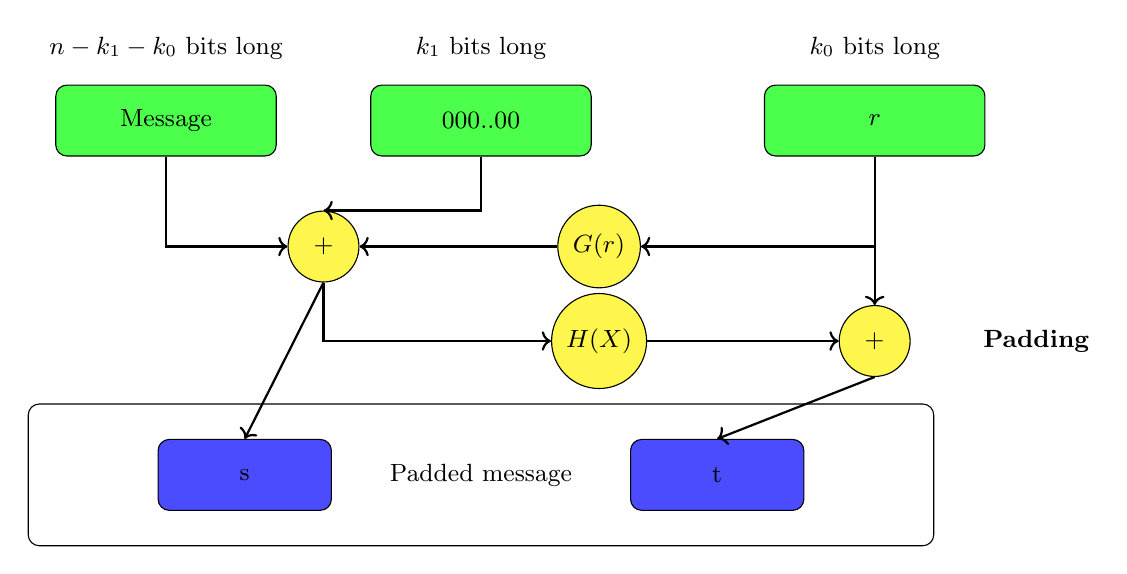
\begin{tikzpicture}[
		font=\small,
		box/.style={draw, rectangle, rounded corners, minimum width=28mm, minimum height=9mm, fill=green!70},
		op/.style={draw, circle, minimum size=9mm, fill=yellow!70},
		var/.style={draw, rectangle, rounded corners, minimum width=22mm, minimum height=9mm, fill=blue!70},
		arrow/.style={->, thick},
		node distance=14mm and 24mm
		]
		
		% Bit-length labels
		\node at (0,4.1) {$n$ bits long};
		
		% Top input blocks
		\node[box] (msg) at (-4,4) {Message};
		\node[above=2mm of msg] {$n-k_1-k_0$ bits long};
		
		\node[box] (zeros) at (0,4) {000..00};
		\node[above=2mm of zeros] {$k_1$ bits long};
		
		\node[box] (r) at (5,4) {$r$};
		\node[above=2mm of r] {$k_0$ bits long};
		
		% First XOR
		\node[op] (xor1) at (-2,2.4) {$+$};
		
		\draw[arrow] (msg.south) |- (xor1.west);
		\draw[arrow] (zeros.south) |- (xor1.north);
		
		% G(r)
		\node[op] (G) at (1.5,2.4) {$G(r)$};
		\draw[arrow] (r.south) |- (G.east);
		\draw[arrow] (G.west) -- (xor1.east);
		
		% H(X)
		\node[op] (H) at (1.5,1.2) {$H(X)$};
		\draw[arrow] (xor1.south) |- (H.west);
		
		% Second XOR
		\node[op] (xor2) at (5,1.2) {$+$};
		\draw[arrow] (H.east) -- (xor2.west);
		\draw[arrow] (r.south) -- (xor2.north);
		
		% Padded message container
		\node[draw, rectangle, rounded corners, minimum width=115mm, minimum height=18mm] (pad) at (0,-0.5) {};
		\node at (0,-0.5) {Padded message};
		
		% X and Y blocks
		\node[var] (X) at (-3,-0.5) {s};
		\node[var] (Y) at (3,-0.5) {t};
		
		\draw[arrow] (xor1.south) -- (X.north);
		\draw[arrow] (xor2.south) -- (Y.north);
		
		% Padding label
		\node[right=8mm of xor2] {\textbf{Padding}};
		
	\end{tikzpicture}
	
	That is:
	\begin{align}
		s &= m \oplus G(r)\\
		t &= r \oplus H(s)
	\end{align}
	and $\hat{m} = s || t$, and encrypt $\hat{m}$ with RSA.
	
	\section{Summary of learnt public key encryption schemes so far}
	
	\begin{table}[h]
		\centering
		\begin{tabular}{|l|c|c|}
			\hline
			\textbf{Property} & \textbf{ElGamal} & \textbf{RSA} \\
			\hline
			Security parameter & $n$ & $n$ \\
			\hline
			Public keys & $p, g, g^x$ & $N, e$ \\
			\hline
			Public key size & $3n$ & $2n + c$ \\
			\hline
			Secret key & $x$ & $d$ \\
			\hline
			Secret key size & $n$ & $n$ \\
			\hline
			Ciphertext & $(g^y, g^{xy}\cdot m)$ & $m^e \bmod N$ \\
			\hline
			Ciphertext size & $2n$ & $n$ \\
			\hline
		\end{tabular}
		\caption{Comparison of ElGamal and RSA public key encryption schemes}
	\end{table}
	
	\section{Digital signatures}
	
	\begin{definition}[Digital signature scheme]
		\leavevmode
		A digital signature scheme $\Pi$ consists of three PPT algorithms: $\Pi = (\Gen, \Sig, \Ver)$.
		\begin{itemize}
			\item $\Gen$:
			\begin{itemize}
				\item Input: $1^n$
				\item Output: $pk, sk$
			\end{itemize}
			\item $\Sig$:
			\begin{itemize}
				\item Input: $m, sk$
				\item Output: $\sigma \leftarrow \Sig_{sk}(m)$
			\end{itemize}
			\item $\Ver$:
			\begin{itemize}
				\item Input: $\sigma, pk, m$
				\item Output: $b =
				\begin{cases}
					1, \text{if valid}\\
					0, \text{if invalid}
				\end{cases}$
			\end{itemize}
		\end{itemize}
		We require, except with negligible probability, that $\Ver_{pk}(m, \Sig_{sk}(m)) = 1$.
	\end{definition}
	
	\begin{definition}[Security of a digital signature scheme]
		\leavevmode
		\begin{itemize}
			\item Adversary $A$ knows the public parameters $\Pi, pk$.
			\item $A$ knows many $(m, \sigma)$ pairs.
		\end{itemize}
		Our goal is to prevent a PPT adversary $A$ to obtain the following:
		\begin{itemize}
			\item A signature of a \emph{new} message $m$.
			\item A \emph{new} signature of an \emph{old} message.
		\end{itemize}
		We do \emph{not} care about replay attacks.
	\end{definition}
	
	\begin{definition}[The signature forging experiment]
		The signature forging experiment $\text{Sig-forge}_{A, \Pi}(n)$ is the following:
		\begin{enumerate}
			\item Run $G(1^n)$ to obtain $(pk, sk)$
			\item $A$ is given $pk$, and oracle access to $\Sig_{sk}(.)$
			\item Let $Q$ be the set of all queries that $A$ submitted to the oracle and also the oracle's answers.
			\item $A$ outputs $(m, \sigma)$.
			\item $\text{Sig-forge}_{A, \Pi}(n) =
			\begin{cases}
				1, if \Ver(m, \sigma) = 1 \cap (m, \sigma) \not \in Q \\
				0 \text{ otherwise}
			\end{cases}$
		\end{enumerate}
	\end{definition}
	
	\begin{definition}[Security of a digital signature scheme]
		A digital signature scheme $\Pi(\Gen, \Sig, \Ver)$ is secure if for all PPT adversary A:
		$$
		\Pr[\text{Sig-forge}_{A, \Pi}(n) = 1] \le \negl(n)
		$$
	\end{definition}
	
	\subsection{The RSA-signature scheme}
	
	\begin{definition}[Plain RSA-signature scheme]
		\item $\Gen$:
		\begin{itemize}
			\item Input: $1^n$
			\item Output: $pk = (N, e), sk = d$ as in RSA.
		\end{itemize}
		\item $\Sig$:
		\begin{itemize}
			\item Input: $m \in \mathbb{Z}_n^*, sk = d$
			\item Output: $m, \sigma = m^d \pmod{N}$
		\end{itemize}
		\item $\Ver$:
		\begin{itemize}
			\item Input: $(m, \sigma), pk = (N, e)$
			\item Output: Verifies, whether $m = \sigma^e \pmod{N}$
		\end{itemize}
	\end{definition}
	
	\begin{remark}
		For a given $m$, it is as hard to obtain $\sigma$ and breaking RSA. However, one can easily generate valid $(m, \sigma)$ pairs: If $A$ knows at least two documents and corresponding signatures $(m_1, \sigma_1), (m_2, \sigma_2)$, then $(m, \sigma) = (m_1m_2, \sigma_1\sigma_2)$ is also valid: $m^d = (m_1m_2)^d = m_1^dm_2^d=\sigma_1\sigma_2$.
	\end{remark}
	
	\begin{definition}[RSA-FDH (Full Domain Hash) signature]
		\leavevmode
		\begin{itemize}
			\item Let $H: \{0, 1\}^* \rightarrow \mathbb{Z}_N^*$ be a hash function.
			\item $\Gen$:
			\begin{itemize}
				\item Input: $1^n$
				\item Output: $pk = (N, e), sk = d$
			\end{itemize}
			\item $\Sig$:
			\begin{itemize}
				\item Input: $m, sk$
				\item Output: $m, \sigma = H(m)^d$
			\end{itemize}
			\item $\Ver$:
			\begin{itemize}
				\item Input: $m, \sigma, pk$
				\item Output: $H(m) = \sigma^e \pmod{N}$
			\end{itemize}
		\end{itemize}
	\end{definition}
	
	\begin{remark}
		One can prove the security of this scheme. It is also called the hash-and-sign paradigm.
	\end{remark}
		
\end{document}
